\subsection{Heat-ball mean values (Evans \S2.3.2, Theorem 3)}
\label{sec:2-heatball}
We now expand the connection with harmonic means. The region, the time
orientation, and the weight are all essential.

\subsubsection*{1. The kernel determines the geometry}
Let $K(z,\tau)=(4\pi\tau)^{-n/2}e^{-|z|^2/(4\tau)}$, $\tau>0$.
For a target $(x,t)$ define
\[
 E_r(x,t)=\{(y,s):s<t,\ K(x-y,t-s)>r^{-n}\}.
\]
The open or closed choice on the ordinary boundary does not affect
the integral. Put $\tau=t-s$ and $a=r^2/(4\pi)$.
Taking logarithms gives
\[
 0<\tau<a,\qquad |y-x|<R_r(\tau),\qquad
 R_r(\tau)^2=2n\tau\log(a/\tau).
 \tag{HB}
\]
Each past slice is an ordinary spatial ball. Its radius vanishes at both
tips and is largest at $\tau=a/e$:
\[
 \max R_r(\tau)=r\sqrt{\frac n{2\pi e}}.
\]
Thus $r$ is a kernel-level scale, not the largest spatial radius.
\Needspace{45mm}
\PDEAnnotation{热球为何朝向过去}{核 $K(x-y,t-s)$ 只在 $s<t$ 有意义。热球下端在 $t-r^2/(4\pi)$，上端是目标时刻 $t$；它不是以 $(x,t)$ 为对称中心的时空球。}
\begin{center}
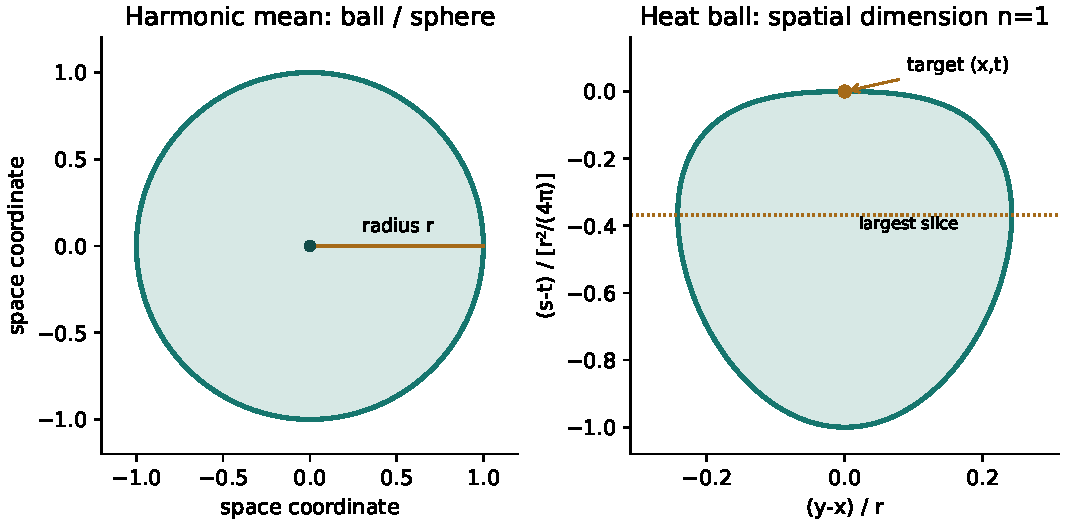
\includegraphics[width=\linewidth]{output/figures/ch02-mean-geometries.pdf}
\end{center}
\noindent\textit{Editorial figure.} Left: an elliptic ball and its boundary.
Right: a one-dimensional spatial section of a heat ball, with time
increasing toward the target. Spatial and temporal axes use different scales.


\PDEBodyDiagram{2.3}{A heat ball carries a nonuniform averaging measure.}
{In one spatial dimension, fix a past time $\tau=t-s$. The blue band marks the allowed interval, while orange heights illustrate the factor $z^2/(4r\tau^2)$. The right panel shows its quadratic spatial dependence up to a fixed positive factor. This is a slice of the full space--time probability measure, not a separately normalized conditional density.}
{ch02-heatball-weight}

\subsubsection*{2. Statement and full proof}
\begin{theorem}[Watson--Evans mean-value formula]\label{thm:2-heatmean}
If $u\in C^{2,1}$ solves $Lu=u_t-\Delta u=0$ on a neighborhood of
$\overline E_r(x,t)$, then
\[
 \boxed{u(x,t)=\frac1{4r^n}\iint_{E_r(x,t)}
 u(y,s)\frac{|x-y|^2}{(t-s)^2}\,dy\,ds.}
 \tag{H}
\]
The nonnegative measure
\[
 d\mu_r(y,s)=\frac{\mathbf1_{E_r(x,t)}}{4r^n}
                    \frac{|x-y|^2}{(t-s)^2}\,dy\,ds
\]
has mass one, so this is $u(x,t)=\mathbb E_{\mu_r}[u(Y,S)]$.
\end{theorem}
\Needspace{45mm}
\PDEAnnotation{区域和权重缺一不可}{均匀热球抽样使用 $dy\,ds/|E_r|$；这里使用 $|x-y|^2/[4r^n(t-s)^2]$。即使区域画对了，丢掉权重仍然不是均值定理。}

\begin{expandedproof}[including the source's omitted normalization]
\paragraph{A. Compute the mass exactly.}
At fixed $\tau$, $\int_{B_R}|z|^2\,dz=n\omega_n R^{n+2}/(n+2)$.
With $b=n/2$ and $a=r^2/(4\pi)$, polar integration gives
\[
 \begin{split}
 I_r&:=\iint_{E_r(0,0)}\frac{|y|^2}{s^2}\,dy\,ds\\
 &=\frac{n\omega_n}{n+2}(2n)^{b+1}
 \int_0^a\tau^{b-1}[\log(a/\tau)]^{b+1}\,d\tau .
 \end{split}
\]
Set $q=\log(a/\tau)$, so $\tau=ae^{-q}$. Then
\[
 \int_0^a\tau^{b-1}[\log(a/\tau)]^{b+1}\,d\tau
 =a^b\int_0^\infty e^{-bq}q^{b+1}\,dq
 =a^b\frac{\Gamma(b+2)}{b^{b+2}}.
\]
Here $\Gamma(c)=\int_0^\infty z^{c-1}e^{-z}\,dz$;
the last equality uses $z=bq$.
Substitute $\omega_n=\pi^b/\Gamma(b+1)$,
$a^b=r^n/(4\pi)^b$, and $\Gamma(b+2)=(b+1)\Gamma(b+1)$.
Cancellation yields
\[
 I_r=4r^n,\qquad \mu_r(E_r)=1.
\]
This also proves integrability of the seemingly singular top-tip weight
for every $n\geq1$.

\paragraph{B. Differentiate after fixing the domain.}
Translate the target to $(0,0)$; thus integration times $s$ are negative.
Scaling of $K$ gives $E_r=\{(ry,r^2s):(y,s)\in E_1\}$.
Define
\[
 \phi(r)=r^{-n}\iint_{E_r}u(y,s)\frac{|y|^2}{s^2}\,dy\,ds
 =\iint_{E_1}u(ry,r^2s)\frac{|y|^2}{s^2}\,dy\,ds.
\]
The Jacobian is $r^{n+2}$ and the weight contributes $r^{-2}$,
explaining the cancellation. First suppose $u$ smooth.
Differentiate on $E_1$, then scale back:
\[
 \phi'(r)=A+B,
\]
\[
 A=r^{-n-1}\iint_{E_r}(y\cdot Du)\frac{|y|^2}{s^2},\qquad
 B=r^{-n-1}\iint_{E_r}2u_s\frac{|y|^2}{s}.
 \tag{AB}
\]
Bounded derivatives on compact sets and the integrable weights justify
this operation for radii in a compact admissible interval.

\paragraph{C. Find a boundary-vanishing function.}
Set
\[
 \psi_r=\log\big(r^nK(y,-s)\big)
 =n\log r-\frac n2\log(-4\pi s)+\frac{|y|^2}{4s}.
\]
It is positive inside $E_r$, zero on its lateral boundary, and
\[
 D_y\psi_r=\frac{y}{2s},\qquad
 (\psi_r)_s=-\frac n{2s}-\frac{|y|^2}{4s^2}.
 \tag{L}
\]
Since $2|y|^2/s=4y\cdot D\psi_r$, spatial integration by parts gives
\[
 B=-4r^{-n-1}\iint_{E_r}\psi_r(nu_s+y\cdot Du_s).
\]
Integrate the last term in time and insert (L):
\[
 \begin{split}
 B&=r^{-n-1}\iint_{E_r}
       [-4n\psi_ru_s+4(\psi_r)_s\,y\cdot Du]\\
 &=-4nr^{-n-1}\iint_{E_r}\psi_ru_s
   -2nr^{-n-1}\iint_{E_r}\frac{y\cdot Du}{s}-A.
 \end{split}
\]
The $A$ terms cancel. Use $y/s=2D\psi_r$ and integrate spatially once more:
\[
 \boxed{\phi'(r)=4nr^{-n-1}
                 \iint_{E_r}\psi_r(\Delta u-u_s).}
 \tag{R}
\]
For a caloric function the right side is zero, so $\phi$ is constant.

\paragraph{D. Check both tips and the regularity assumption.}
Zero lateral values alone do not justify ignoring the singular tip.
First truncate to $\varepsilon<\tau<a-\eta$.
The lateral terms vanish because $\psi_r=0$.
At the top cap,
$R=O(\sqrt{\tau\log(a/\tau)})$ and
\[
 \int_{B_R}|y|\psi_r\,dy
 \leq C R^{n+1}\log(a/\tau)\longrightarrow0.
\]
This controls the time-boundary term containing $y\cdot Du$.
At the lower cap, $R\to0$ and $\psi_r\to0$, so that term also vanishes.
The weight remaining near the upper tip is bounded by a constant times
\[
 \int_0^\varepsilon
 \tau^{n/2-1}[\log(a/\tau)]^{n/2+1}\,d\tau\longrightarrow0.
\]
The differentiated terms in (AB) and those with $\psi_r$ have the same
integrable powers or better ones. Let $\varepsilon,\eta\downarrow0$.

For only $C^{2,1}$ regularity, convolve in space-time on a slightly larger
neighborhood. The constant-coefficient operator $L$ commutes with
convolution, so smooth approximations still solve the equation where
needed. They converge uniformly on the compact region; the integrable
weight passes the established mean identity to $u$.
This avoids requiring mixed third derivatives in the original function.
At a terminal cylinder time, take limits from interior target times.

\paragraph{E. Identify the constant by shrinking.}
The heat ball lies in $|y|\leq C_nr$, $|s|\leq r^2/(4\pi)$.
Uniform continuity and the mass computation imply
$\phi(r)\to4u(0,0)$ as $r\downarrow0$.
Therefore $\phi(r)=4u(0,0)$ for every admissible radius.
Divide by four and restore the target $(x,t)$.
\end{expandedproof}
\Needspace{45mm}
\PDEAnnotation{对数核为何出现}{$\psi_r$ 的零边界值消掉侧边界项；空间梯度产生平均权重；时间导数让缩放导数的两项抵消。这三种作用共同决定热球的定义。}

\subsubsection*{3. The precise connection to elliptic averages}
For general smooth $u$ let $M_r[u]=\phi(r)/4$.
The preceding computation, before imposing the PDE, gives
\[
 \frac d{dr}M_r[u](x,t)
 =-\frac n{r^{n+1}}\iint_{E_r(x,t)}
 \log\big(r^nK(x-y,t-s)\big)\,Lu(y,s)\,dy\,ds.
 \tag{HR}
\]
Thus $Lu\leq0$ implies $M_r[u]$ nondecreasing, and shrinking $r$ gives
$u(x,t)\leq M_r[u](x,t)$. Reverse the signs for supersolutions.
This parallels $\Delta v\geq0$ and $\partial_rS_v\geq0$ in (M).
\Needspace{45mm}
\PDEAnnotation{两个次解的符号}{椭圆次调和是 $\Delta v\geq0$，即 $-\Delta v\leq0$；抛物次解是 $v_t-\Delta v\leq0$。统一算子符号后，两者都是“中心不超过正权平均”。}

\paragraph{A counterexample to unweighted replacements.}
The polynomial $u(y,s)=|y-x|^2+2n(s-t)$ has $Lu=0$ and $u(x,t)=0$.
At time $t$ its uniform spatial ball average is $nr^2/(n+2)>0$.
On $B_r(x)\times(t-r^2,t)$ its uniform space-time average is
$nr^2/(n+2)-nr^2\ne0$.
A symmetric Euclidean space-time ball cancels the time term but still
leaves a positive spatial square. None of these is the required mean.
\Needspace{45mm}
\PDEAnnotation{最简单的公式自检}{$|y-x|^2+2n(s-t)$ 的空间曲率与时间变化恰好平衡。正确权重必须把二者抵消；普通空间平均看不到时间补偿。}

\paragraph{Stationary solutions.}
If $u(y,s)=h(y)$, then $Lu=0$ is exactly $\Delta h=0$.
At fixed $\tau$, the heat-ball weight is radial in $y-x$.
Integrate over spherical shells first: every spherical mean of $h$
equals $h(x)$, and the remaining scalar integral is the total mass one.
Thus heat-ball averaging of a stationary solution is an aggregate of
elliptic sphere averages. A time-dependent caloric solution needs the
past slices as well as the weight.

\paragraph{Moments and a converse: editorial supplement.}
There is an exact probability description of $\mu_r$.
Put $b=n/2$, $a=r^2/(4\pi)$.
Let $Q$ have Gamma density proportional to $q^{b+1}e^{-bq}$, $q>0$,
and set $\tau=ae^{-Q}$.
Conditional on $\tau$, choose a uniform direction and radius
$\varrho=R_r(\tau)U^{1/(n+2)}$, with $U$ uniform on $(0,1)$.
Step A gives the time density after the logarithmic substitution.
The conditional spatial radial density is proportional to
$\varrho^{n+1}$, because the volume Jacobian contributes
$\varrho^{n-1}$ and the weight contributes $\varrho^2$.
Hence this construction samples the actual weighted measure.

Gamma integration and symmetry yield
\[
 \mathbb E(Y_i-x_i)=0,\qquad
 \mathbb E[(Y_i-x_i)(Y_j-x_j)]=2\delta_{ij}\mathbb E\tau,
\]
\[
 \mathbb E\tau=c_nr^2,\qquad
 c_n=\frac1{4\pi}\left(\frac n{n+2}\right)^{n/2+2}>0.
\]
For the second moment, conditional radial integration gives
$\mathbb E(|Y-x|^2\mid\tau)
=[(n+2)/(n+4)]\,2n\tau Q$.
Integrating the Gamma density then gives
$\mathbb E|Y-x|^2=2n\mathbb E\tau$.
Taylor expansion for $C^{2,1}$ functions therefore implies
\[
 M_r[u](x,t)=u(x,t)+c_nr^2(\Delta u-u_t)(x,t)+o(r^2).
 \tag{HT}
\]
The remainder is uniform on the shrinking region, and
$\mathbb E(|Y-x|^2+\tau)=O(r^2)$ controls its integral.
An exact identity for all small radii at every center forces $Lu=0$.
Compare this with the elliptic expansion (T).
\Needspace{45mm}
\PDEAnnotation{几何平均在检测算子}{球面平均的二阶误差是 $r^2\Delta u/(2n)$；热球平均的二阶误差是 $c_nr^2(\Delta u-u_t)$。两种几何平均分别检测各自的 PDE。}

\paragraph{Do not confuse this with Gaussian averaging.}
At a fixed earlier time $s$, the whole-space solution can be written
$u(x,t)=\int K(x-y,t-s)u(y,s)\,dy$ in a class where the Cauchy problem
is unique. That is a global spatial Gaussian average on one time slice.
Heat-ball averaging is local in space-time and uses many past slices.
The fundamental solution is the same; the two averaging measures differ.
